\documentclass[12pt,a4paper]{article}
\usepackage{url}            % Pour citer les adresses web
\usepackage[T1]{fontenc}    % Encodage des accents (affichage des accents)
\usepackage[utf8]{inputenc} % Lui aussi (lecture des accents)
\usepackage[french]{babel} % Pour la traduction française
\usepackage{numprint}       % Histoire que les chiffres soient bien

\usepackage{amsmath}        % La base pour les maths
\usepackage{mathrsfs}       % Quelques symboles supplémentaires
\usepackage{amssymb}        % encore des symboles.
\usepackage{amsfonts}       % Des fontes, eg pour \mathbb.

\usepackage[svgnames]{xcolor} % De la couleur
\usepackage{geometry}       % Gérer correctement la taille
\usepackage{array}
\usepackage{curves}
\usepackage{epic}
\usepackage{eepic}
\usepackage{epsfig}
\usepackage{graphics}
\usepackage{minted} % pour Python

%%% Si jamais vous voulez changer de police: décommentez les trois 
%\usepackage{tgpagella}
%\usepackage{tgadventor}
%\usepackage{inconsolata}

%%% Pour L'utilisation de Python
\usepackage{pythontex}

\usepackage{graphicx} % inclusion des graphiques
\usepackage{wrapfig}  % Dessins dans le texte.

\usepackage{tikz}     % Un package pour les dessins (utilisé pour l'environnement {code})
\usepackage[framemethod=TikZ]{mdframed}
% Un environnement pour bien présenter le code informatique
\newenvironment{code}{%
\begin{mdframed}[linecolor=Green,innerrightmargin=30pt,innerleftmargin=30pt,
backgroundcolor=Black!5,
skipabove=10pt,skipbelow=10pt,roundcorner=5pt,
splitbottomskip=6pt,splittopskip=12pt]
}{%
\end{mdframed}
}

% Mettez votre titre et votre nom ci-après
\title{Guide de survie en \LaTeX{}}
\author{Jean-Julien \textsc{Fleck}, PCSI\oldstylenums{1}, \oldstylenums{2016}-\oldstylenums{2017}}
%% À décommenter si vous ne voulez pas que la date apparaisse explicitement
%\date{}

% Un raccourci pour composer les unités correctement (en droit)
% Exemple: $v = 10\U{m.s^{-1}}$
\newcommand{\U}[1]{~\mathrm{#1}}

% Pour discuter avec le prof dans le document: le premier argument est 
% le nom de celui qui fait la remarque et le second la remarque 
% proprement dite: \question{jj}{Que voulez-vous dire par là ?}
% \reponse{Droopy}{I'm very happy...}
\usepackage{todonotes}
\newcommand{\question}[2]{\todo[inline,author=#1]{#2}}
\newcommand{\reponse}[2]{\todo[inline,color=green,author=#1]{#2}}

% Les guillemets \ofg{par exemple}
\newcommand{\ofg}[1]{\og{}#1\fg{}}
% Le d des dérivées doit être droit: \frac{\dd x}{\dd t}
\newcommand{\dd}{\text{d}}


% NB: le script TeXcount permet de compter les mots utilisés dans chaque section d'un document LaTeX. Vous en trouverez une version en ligne à l'adresse
% http://app.uio.no/ifi/texcount/online.php
% Il suffit d'y copier l'ensemble du présent document (via Ctrl-A/Ctrl-C puis Ctrl-V dans la fenêtre idoine) pour obtenir le récapitulatif tout en bas de la page qui s'ouvre alors.

% Pour récupérer les bonnes entrées bibliographiques, je vous conseille l'usage de scholar.google.fr pour les recherches
% et la récupération des entrée BibTeX comme décrit dans cette vidéo: https://www.youtube.com/watch?v=X-9T2Oaj-5A

% Quelques macros  
% La dérivée temporelle, tellement courante en physique, avec les d droits
\newcommand{\ddt}[1]{\frac{\dd #1}{\dd t}}
% Des parenthèses, crochets et accolades qui s'adaptent automatiquement à la taille de ce qu'il y a dedans
\newcommand{\pa}[1]{\left(#1\right)}
\newcommand{\pac}[1]{\left[#1\right]}
\newcommand{\paa}[1]{\left\{#1\right\}}
% Un raccourci pour écrire une constante
\newcommand{\cte}{\text{C}^{\text{te}}}
% Pour faire des indices en mode texte (comme les énergie potentielles)
\newcommand{\e}[1]{_{\text{#1}}}
% Le produit vectoriel a un nom bizarre:
\newcommand{\vectoriel}{\wedge}

% Pour aider à écrire les commandes
\newcommand{\env}[1]{\texttt{\{#1\}}}
\newcommand{\cmd}[1]{\texttt{\textbackslash#1}}
\newcommand{\cmdone}[2]{\cmd{#1\{\emph{#2}\}}}


\begin{document}

\maketitle


\begin{abstract}

%	Find something meaningful to say in english in order to describe the present report...
    
    Ce document va essayer de vous présenter les principes fondamentaux de l'écriture d'un document \LaTeX{} en essayant d'éviter les écueils habituellement rencontrés par les néophytes. Ce premier environnement qui sert à mettre votre résumé (\emph{a priori} en anglais pour le TIPE) s'appelle \env{abstract}.
    
    Attention à ce que votre résumé soit effectivement un \emph{résumé} rapide de votre travail et non une introduction littéraire.
    
\end{abstract}

\section{Ne confondez pas \LaTeX{} avec Word...}

Le point principal est que l'on ne dit pas à \LaTeX{} \emph{comment} il doit afficher quelque chose, mais \emph{ce qu'on voudrait} qu'il affiche. Il sait faire son boulot, donc laissez-le faire et concentrez-vous sur le \emph{fond} et non sur la \emph{forme}. Quelques exemples à venir:


\subsection{Titres et structuration du document}

Pour faire des titres de section, utilisez la commande \cmdone{section}{Mon titre de section} où, bien sûr, vous remplacez \ofg{\emph{Mon titre de section}} par le titre que vous voudriez mettre. \LaTeX{} s'occupe tout seul de la numérotation, il y a moyen de changer le mode de numérotation (chiffres romains par exemple), il suffit de demander gentiment, mais pour le moment, je vous le déconseille.

Bien sûr, on peut faire des sous-sections\footnote{Et même des sous-sous-sections avec \cmdone{subsubsection}{Ma sous-sous-section}, mais la sous-sous-sous-section n'existe pas par défaut, vous pouvez utiliser \cmdone{paragraph}{Mon entame de paragraphe} si vraiment vous en avez besoin.} à l'aide de la commande idoine: \cmdone{subsection}{Mon titre de sous-section}, où là aussi, il suffit de changer l'argument de la commande avec ce que vous voulez.

\subsection{Énumérations}

Il existe plusieurs type d'énumérations:
\begin{itemize}
	\item	les non numérotées (comme celle-ci) que l'on compose dans l'environnement \env{itemize}, chaque nouvel élément étant introduit par la commande \cmd{item}.
    
    \item	les numérotées (\LaTeX{} s'occupant automatiquement de la numérotation) à l'aide de l'environnement \env{enumerate}:
    	\begin{enumerate}
        	\item	Mon premier item ; 
            
            \item	Mon second item, on peut même sous-numéroter
            	\begin{enumerate}
                	\item	mon premier sous-item ;
                    
                    \item	mon second.
                \end{enumerate}
            
            \item	Mon troisième item.
            
        \end{enumerate}
    \item	il existe aussi des énumérations un peu spéciales qui se nomment des \ofg{descriptions} et, sans surprise, elles se composent à l'aide de l'environnement \env{description} avec la particularité de devoir donner un argument optionnel à la commande \cmd{item[\emph{argument optionnel}]}. Par exemple
    	\begin{description}
        	\item[Préambule:] Là où l'on met les déclarations de commandes et imports de modules.
            
            \item[Corps du document:] le corps du texte, là où on écrit les choses intéressantes qui seront affichées à l'écran
            
            \item[Postambule:] ce qui est mis après le \cmd{end\{document\}} est purement et simplement ignoré, ce qui peut servir pour débusquer un bug en rajoutant justement la commande \cmd{end\{document\}} à divers endroits (en partant de la fin) jusqu'à ce que le document compile correctement.
        \end{description}
    
\end{itemize}

\subsection{Paragraphes}

Pour passer à un nouveau paragraphe, il suffit de sauter une ligne dans le fichier source et \LaTeX{} s'occupe tout seul de commencer un nouveau paragraphe avec l'indentation adéquate.

Si pour une raison ou une autre, vous voudriez qu'il n'y ait pas d'indentation pour le nouveau paragraphe (par exemple si vous continuez une phrase après une équation centrée), il suffit de le demander gentiment à \LaTeX{} avec l'instruction \cmd{noindent} donnée après avoir sautée votre ligne dans le fichier source, mais sans sauter de ligne avant la suite de votre prose

\noindent comme je vient de le faire ici.

Il peut arriver que vous vouliez \emph{effectivement} sauter une ligne dans le rendu visuel de votre document\footnote{Quelle drôle d'idée... On vous a pourtant dit de laisser \LaTeX{} s'occuper de tout !}, vous pouvez alors utiliser l'une ou l'autre des commandes \cmd{smallskip}, \cmd{medskip} ou \cmd{bigskip} en sautant deux lignes autour de deux nouveaux paragraphes

\bigskip

comme je viens de le faire ici, mais bon, on vous le répète, ce n'est pas une bonne idée en général de se concentrer sur la forme: vous devez vous occuper du fond et laisser \LaTeX{} gérer la forme !

\subsection{Mise en page finale}

Lorsque vous êtes sûr que votre texte ne va plus évoluer (ou seulement aux détails près), vous pouvez commencer à vous demander si les sauts de pages sont bien placés\footnote{Mais seulement à ce moment là, c'est-à-dire quelques heures avant de rendre votre travail !}. Il y a deux commandes principales permettant de gérer les sauts de page: 
\begin{description}	
    \item[\cmd{newpage}] qui arrête purement et simplement la composition de la page courante au point où elle est placée et en commence une nouvelle
    
    \item[\cmd{eject}] qui essaie, si c'est possible, d'étendre les espaces verticaux pour que l'on ait tout de même l'impression que la page est entièrement remplie avant de passer à la suivante.

\end{description}

\section{Le texte}

\subsection{Changer de police}

Oubliez... Un document \LaTeX{} n'est pas un sapin de Noël... C'est par le fond que vous allez convaincre votre interlocuteur de la pertinence de votre propos et non grâce à des contorsions typographiques. Si vraiment vous voulez changer la police par défaut (qui est caractéristique d'un document \LaTeX, il est vrai, mais vous ne serez pas tant que cela dans ce cas \emph{a priori}), vous pouvez décommenter les lignes suivantes normalement présentes dans le préambule du template que je vous ai préparé

\begin{code}
\begin{verbatim}
\usepackage{tgpagella}
\usepackage{tgadventor}
\usepackage{inconsolata}
\end{verbatim}
\end{code}

\subsection{Varier la fonte}

En revanche, il est bon de pouvoir mettre certains passages de votre texte en exergue, que ce soit en \textbf{gras} (à l'aide de la commande \cmdone{textbf}{Texte en gras}) ou en \textit{italique} (à l'aide de la commande \cmdone{textit}{Texte en italique}).

À noter que la commande \cmdone{emph}{Texte à mettre en relief} (qui vient de l'anglais \emph{emphasize}) regarde le contexte alentour pour mettre le texte en \emph{italique} si la fonte est normale autour ou \textit{le mettre en caractères \emph{droits} si le texte autour est déjà en italique, ce qui assure que le mot ressorte correctement du paragraphe}.

\subsection{Notes en bas de page}

Il est possible de mettre des jalons pour des notes en bas de page à l'aide de la commande \cmdone{footnote}{Texte de la note.} à coller directement au texte qui suit\footnote{sinon un espace en trop est inséré entre la dernière lettre du mot et l'exposant signalant la note.} comme ceci


\begin{code}
\begin{verbatim}
à coller directement au texte qui suit\footnote{sinon un 
espace en trop est inséré entre la dernière lettre du mot 
et l'exposant signalant la note.} comme ceci
\end{verbatim}
\end{code}

\subsection{Guillemets et caractères spéciaux}

Dans le préambule de ce document, la macro \cmdone{ofg}{entre guillemets} (pour \ofg{Ouvrir et Fermer les Guillemets}) a été définie. Elle s'assure que l'on compose bien les guillemets \ofg{à la française} et non "à l'anglaise".

En outre, il existe dans la langue française quelques caractères un peu bizarre comme le \ofg{o dans l'e} que l'on compose à l'aide de la commande \cmd{oe\{\}} comme dans le mot \verb|n\oe{}ud| qui ressort alors sous la forme \ofg{n\oe{}ud} et non \ofg{noeud}. De la même manière, le \c{c} se compose \verb|\c{c}|

\section{Les mathématiques}

\subsection{Du bon usage des dollars}

\emph{Tout} texte mathématique doit se trouver en \ofg{mode mathématique}, c'est-à-dire la plupart du temps entre dollars. Il faut distinguer 
	\begin{itemize}
    	\item le comportement entre dollars simples à utiliser à l'intérieur du texte par exemple pour parler d'une fonction $f$ (\verb|$f$|) de la variable $x$ (\verb|$x$|), ce qui est bien plus propre que de parler de la fonction f de la variable x\footnote{Arrivez-vous à voir la différence ? C'est pourtant flagrant.}...
        \item du comportement entre dollars doubles qui, même s'il est utilisé dans un paragraphe de texte, va centrer la formule mathématique sans la numéroter et changer le comportement de certaines commandes pour que le rendu prenne plus de place, par exemple \verb|\frac{a}{b}| donnera $\frac{a}{b}$ 
        entre dollars simples\footnote{À noter que l'on peut forcer l'obtention de \ofg{grandes} fractions dans le texte avec des dollars simples en utilisant 
        \texttt{\$}\cmd{dfrac\{a\}\{b\}\$}
        (pour \ofg{displaystyle fraction}) plutôt que \cmd{frac}.} 
        mais $$\frac{a}{b}$$ entre dollars doubles.
    \end{itemize}

Il est à noter que les dollars sont des primitives de \TeX{} (le moteur du rendu à la base de \LaTeX{}) et \LaTeX{} introduit d'autres notations qui ont eu plus de mal à s'imposer une fois qu'on a pris l'habitude des dollars à savoir
\begin{description}
	\item[\cmd{(} et \cmd{)}] à utiliser lorsqu'on veut mettre des maths dans le texte comme \(\frac{a}{b}\) (composé \verb|\(\frac{a}{b}\)|) en remplacement des dollars simples\footnote{Cette notation a beaucoup de mal à s'imposer car elle a l'inconvénient de demander de taper 2 caractères au lieu d'un...} de \TeX{}.
    \item[\cmd{[} et \cmd{]}] à utiliser pour centrer des équations sans numérotation comme \[\frac{a}{b}\] (composé \verb|\[\frac{a}{b}\]|) en remplacement des dollars doubles\footnote{Là, c'est plus utilisé} de \TeX{}.
\end{description}

\subsection{Bases des notations mathématiques}

Écrire des maths en \LaTeX{} peut sembler un peu hermétique de prime abord, mais cela devient vite une seconde nature pour pouvoir exprimer des symboles compliqué à l'aide de simple texte. Voici les commandes et notations les plus couramment utilisées:
\begin{description}
	
    \item[Indices:] La mise en indice se fait à l'aide du \ofg{tiret-bas} (caractère \texttt{\_}, appelé \emph{undescore} en anglais) comme dans \verb|la suite $(u_n)_{n\in\mathbb{N}}$| qui donne \ofg{la suite $(u_n)_{n\in\mathbb{N}}$}. À noter que si vous ne mettez qu'un unique caractère en indice, on peut omettre de mettre des accolades comme dans \verb|$a_i$| qui donne $a_i$, mais si vous avez besoin de plus de caractères en indices, il suffit de les grouper entre accolades avant de les donner au tiret-bas, par exemple \verb|$M_{ij}$| donne $M_{ij}$.
   	
    \item[Exposants:] Les exposants se composent de la même manière mais en utilisant le chapeau de l'accent circonflexe. Ainsi, \verb|$a^x$| donne $a^x$, \verb|$b^{x\ln(2)}$| donne $b^{x\ln(2)}$, etc. À noter que les règles de typographie impose de différencier les deux notations $\omega_0^2$ (\verb|$\omega_0^2$| oméga indice 0 et exposant 2) de ${\omega_0}^2$ (\verb|${\omega_0}^2$|, oméga 0 à la puissance 2).
    
    \item[Fonctions usuelles:] Les fonctions usuelles doivent être composées en caractères droits en non italiques. Elles ont donc des commandes dédiées: \cmd{cos}, \cmd{sin}, \cmd{tan}, \cmd{exp}, \cmd{ln}, \cmd{log}, etc. $\cos x$, $\sin(\omega t)$, $\tan\varphi$, $\exp(-E_p/k_BT)$, $\log[\mathrm{Cu}^{2+}]$, etc.
    
    \item[Fractions, racines:] Les fractions se composent à l'aide \cmd{frac} qui prend deux arguments (le numérateur puis le dénominateur) et les racines à l'aide de \cmd{sqrt} qui prend en argument ce qui va être sous la racine. Exemple: $$\sqrt{\frac{1 + \frac{2}{3}}{4 + \frac{5}{6}}}$$
    
    \item[Intégrales et dérivées:] Les intégrales se composent à l'aide du symbole \cmd{int} qui prend en indice et en exposant les deux bornes d'intégrations. Pour les dérivées, on préfèrera utiliser un \ofg{d droit} composé à l'aide de la commande \cmd{mathrm} ou en utilisant le raccourci \cmd{dd} défini dans le préambule de ce document (et du template pour le rapport de TIPE)
    
   \[
   \int_a^b \frac{\dd f}{\dd x}\,\dd x = [f(x)]_a^b
   \]
    
    \item[Adapter la taille des parenthèses:] Lorsqu'il y a des parenthèses autour d'une fraction, le rendu de base n'est pas terrible, voyez plutôt le résultat de \verb|\[(\frac{A}{B})\]|
    
    \[(\frac{A}{B})\]
    
    c'est pourquoi, on pourra utiliser le couple de commande \cmd{left} et \cmd{right} dont le caractère suivant est le symbole dont il faut adapter la taille pour l'ajuster à ce qui se trouve entre les deux commandes. Ainsi, l'exemple précédent devient \verb|\[\left(\frac{A}{B}\right)\]|, soit
    
      \[\left(\frac{A}{B}\right)\]
    
    Rien n'empêche a priori de ne pas être cohérent entre l'ouverture et la fermeture, voir par exemple de \verb|\[\left[\sqrt{1 + \f{A}{B}}\right\}\]|
    
    \[\left[\sqrt{1 + \frac{A}{B}}\right\}\]
    
    À noter, que si l'on ne désire par exemple qu'une accolade ouvrante (par exemple pour composer un système), on utilisera le point comme symbole de fermeture qui sera alors vide (\verb|\right.|). Par exemple, le résultat suivant
    
    \[\left\{
    \begin{array}{>{\displaystyle}r@{\ =\ }>{\displaystyle}l}
    \frac{\dd \vec{p}}{\dd t} 	& 	\sum \vec{F}	\\[3mm]
    \frac{\dd E_m}{\dd t}		&	\sum W_{\mathrm{fnc}}
    \end{array}
    \right.\]
    
    a été obtenu à l'aide du code\footnote{Un peu compliqué, mais cela peut vous faire un exemple si jamais}
    
\begin{code}
\begin{verbatim}
\[
\left\{
\begin{array}{>{\displaystyle}r@{\ =\ }>{\displaystyle}l}
\frac{\dd \vec{p}}{\dd t} 	& 	\sum \vec{F}	\\[3mm]
\frac{\dd E_m}{\dd t}		&	\sum W_{\mathrm{fnc}}
\end{array}
\right.
\]
\end{verbatim}
\end{code}
    
    \item[Symbole de multiplication:] On utilisera de préférence \cmd{times} pour représenter une multiplication ($a\times b$ obtenu par \verb|$a\times b$|), mais on peut aussi utiliser \cmd{cdot} qui donne $a\cdot b$ (\verb|$a\cdot b$|, notamment utile pour les produits scalaires).
\end{description}

\subsection{Équations centrées et numérotées}

On n'a pas forcément besoin de numéroter toutes les équations que l'on manipule, mais on doit pouvoir en citer certaines dans le texte sans avoir à se compliquer la vie, ni s'arracher les cheveux si jamais on rajoute une équation numérotée dans l'intervalle\footnote{Après une remarque fort à propos de vos professeurs préférés par exemple...}. Bref, là encore, il faut laisser \LaTeX{} faire le boulot pour vous. On dispose de plusieurs possibilités
	\begin{description}
    	\item[Équation sur une ligne] L'environnement \env{equation} permet de numéroter automatiquement une équation sur une seule ligne. On donne un nom à l'équation à l'aide de la commande \cmd{label} (dont l'argument est le nom en question\footnote{qui ne doit pas contenir d'espace ni d'accent si vous voulez survivre}). Par la suite, on peut y faire référence grâce à la commande \cmd{ref} qui prend en argument le nom que l'on a donné précédemment. Sans rien savoir des équation alentours, je sais que la suivante est la numéro \ref{RFD} puisque c'est le nom que je lui ai donné
        
\begin{equation}
    \ddt{\vec{p}} = \sum \vec{F} 
    \qquad \text{avec} \qquad 
    \vec{p} = m\vec{v} \label{RFD}
\end{equation}

À noter que je peux aussi bien y faire référence avant ou après (c'était l'équation~\ref{RFD}...), \LaTeX{} s'arrangera pour trouver l'information, pourvu que l'on ait compilé suffisamment de fois, ce dont overleaf s'assure. 

\begin{code}
\begin{verbatim}
\begin{equation}
    \ddt{\vec{p}} = \sum \vec{F} 
    \qquad \text{avec} \qquad 
    \vec{p} = m\vec{v} \label{RFD}
\end{equation}
\end{verbatim}
\end{code}

À noter aussi qu'il n'est nul besoin de dollars ici, \LaTeX{} sait qu'il doit basculer en mode math quand on rentre dans un tel environnement.

	\item[Équations sur plusieurs lignes] Quand on veut aligner verticalement plusieurs équations, on peut utiliser l'environnement \env{align} pour lequel on pose des \ofg{jalons} à l'aide de l'esperluette (symbole \texttt{\&}) pour dire à quel endroit on veut l'alignement. On passe d'une ligne à l'autre à l'aide du double backslash (\texttt{\textbackslash\textbackslash}), en donnant en argument optionnel (donc entre crochets) une indication de la longueur qui doit être sautée entre les lignes

\begin{align}
    \ddt{r} 		 &= -\frac{L}{\gamma\, m}\, \frac{\dd u}{\dd \theta} \\[2mm]
    r\, \ddt{\theta} &= \frac{L}{\gamma \, m}\, u \label{binet}
\end{align}

\begin{code}
\begin{verbatim}
\begin{align}
    \ddt{r}          
      &= -\frac{L}{\gamma\, m}\, 
         \frac{\dd u}{\dd \theta} \\[2mm]
    r\, \ddt{\theta} 
      &= \frac{L}{\gamma \, m}\, u \label{binet}
\end{align}
\end{verbatim}
\end{code}

Ici, seule l'équation~\ref{binet} a été pourvue d'un label permettant d'y faire référence, mais elles sont tout de même toutes les deux numérotées. Si on veut empêcher la numérotation d'une seule des deux équations, il suffit de rajouter la commande \cmd{notag} avant le saut de ligne, en lieu et place de la commande \cmd{label}.

    \end{description}

\section{Les figures et tableaux}

\LaTeX{} permet de gérer de manière assez fine le placement des figures, mais le comportement par défaut n'est pas forcément celui auquel vous êtes habitués de prime abord. En effet, dans la littérature scientifique, il est d'usage que les figures se trouvent soit en haut de chaque page, soit en bas, mais en tous cas pas forcément directement à l'endroit où l'on s'attend qu'elles soient, notamment, pas à l'endroit où l'on donne effectivement l'instruction à \LaTeX{} de composer une figure.



\subsection{Introduction d'une figure dans \LaTeX}

L'introduction d'une figure se fait par le biais de l'environnement \texttt{figure} et de la commande \texttt{\string\includegraphics}. Cette commande n'est disponible que dans le paquet \texttt{graphicx} que vous devrez donc appeler en entête du document source. Supposons que l'on ai une image appelée \texttt{image1.jpg} située dans le répertoire de travail. On peut alors ajouter le code suivant :
\begin{code}
\begin{verbatim}
Nous allons mettre une figure
\begin{figure}
\includegraphics{image1.jpg}
\end{figure}
Avez-vous vu notre belle figure?
\end{verbatim}
\end{code}
Bien que la figure soit inclue entre les deux phrases, les phrases seront a priori écrites à la suite. Normal, puisque l'environnement \texttt{figure} est un flottant : \LaTeX{} décide du placement pour que ce soit le \emph{plus joli possible}. On peut cependant forcer un peu la main à \LaTeX{} en ajoutant une option de placement sous la forme \verb!\begin{figure}[t]! pour un affichage en haut de page (\texttt t comme \emph{top}).

Dans un texte scientifique, on s'attachera à toujours inclure une légende sous la figure et à faire référence à la figure dans le texte. Par exemple, la figure~\ref{flottants:exemple:figure}, qui est introduite [ici%
\begin{figure}[b]
\begin{center}
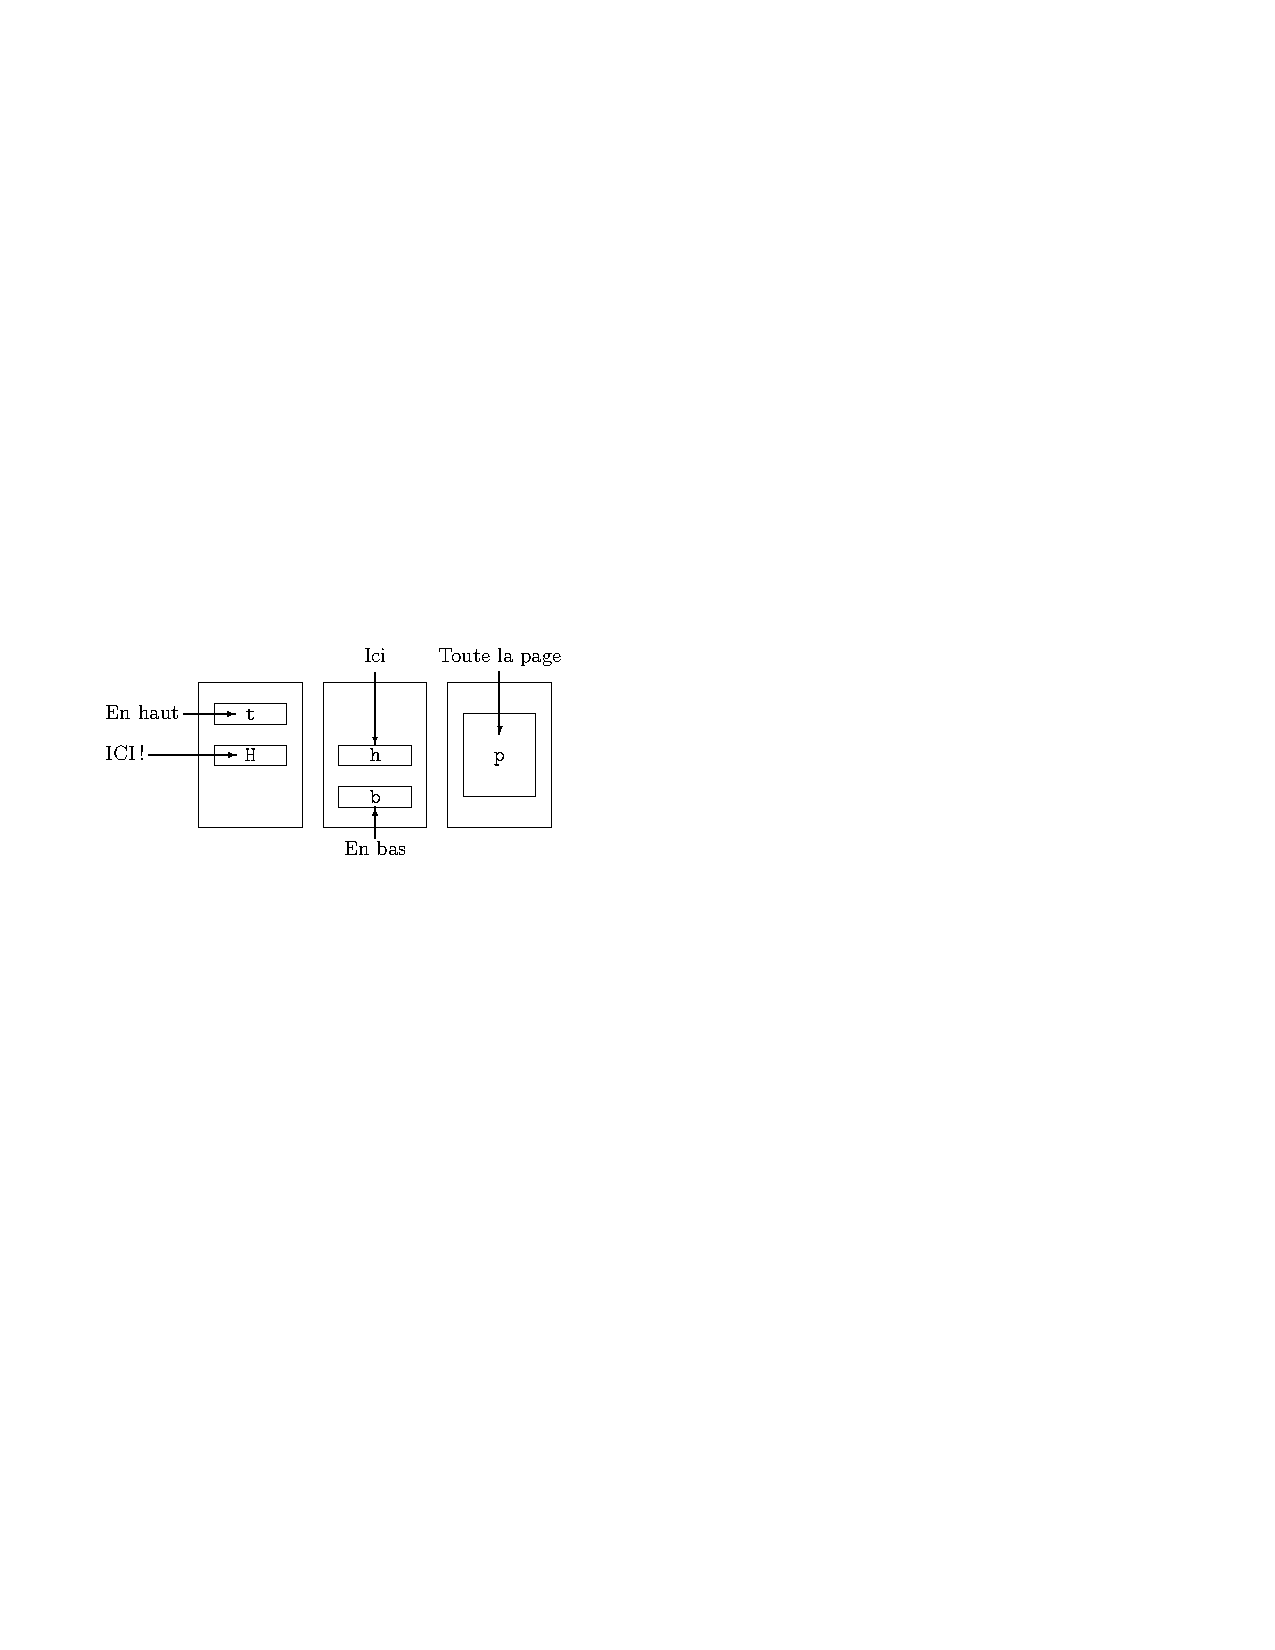
\includegraphics{placement_figures}
\end{center}

\caption{Exemple de flottant: leur placement}\label{flottants:exemple:figure}
\end{figure}%
] dans le code mais s'affiche en bas, rappelle les différentes options de placement des flottants. Essayez tout de même d'aérer votre code en mettant des lignes blanches et en évitant une inclusion au beau milieu d'un paragraphe pour que ce soit un minimum lisible et qu'il n'y ait pas d'espaces introduits de manière inopinée...

On peut aussi vouloir redimensionner la figure pour qu'elle fasse par exemple $50\%$ de la largeur du texte. Nous allons faire tout cela dans l'exemple suivant :

\begin{code}
\begin{verbatim}
\documentclass{report}
\usepackage[utf8]{inputenc}
\usepackage[T1]{fontenc}
\usepackage[french]{babel}
\usepackage{graphicx}


\begin{document}
Nous allons mettre une figure.

\begin{figure}
\includegraphics[width=0.5\textwidth]{image1.jpg}
\caption{Ceci est notre figure}\label{nomdelaref}
\end{figure}

Avez-vous vu notre belle figure \ref{nomdelaref}?
\end{document}
\end{verbatim}
\end{code}

L'option \texttt{width} permet le redimensionnement de la figure en fonction de la longueur prédéfinie \texttt{\string\textwidth}~; on pourrait aussi mettre \texttt{10cm} par exemple. La commande \texttt{\string\label} créé une étiquette pour la figure, la commande \texttt{\string\ref} permet de faire un appel à cette référence. Enfin, la commande \texttt{\string\caption} permet d'afficher une légende. Attention, l'ordre d'écriture entre \texttt{\string\caption} et \texttt{\string\label} est primordial. En effet, la commande \texttt{\string\caption} incrémente un compteur, celui du nombre de figures et la commande \texttt{\string\label} créé une référence au \textsc{dernier} compteur incrémenté. Si vous placez le label avant la légende, vous aurez une référence à la dernière section par exemple... 

Dernier petit point, l'image n'est pas centrée. Contentez-vous d'ajouter \texttt{\string\cen\-te\-ring} juste avant la commande \texttt{\string\includegraphics} et observez le résultat. 

Pour pouvoir afficher plusieurs figures dans la même, avec des références du type \emph{figure 1a)} ou \emph{figure 4c)}, on pourra aller s'intéresser au paquet \texttt{subfigure}.


\subsection{Introduction d'un tableau dans \LaTeX}
Comme l'environnement \texttt{figure}, l'environnement \texttt{table} est un flottant, qui va vous permettre d'insérer un tableau. La différence avec l'environnement \texttt{figure} se trouve dans la légende du flottant : il sera inscrit \emph{Table 1} à la place de \emph{Figure 1}. Nous nous en servons donc pour inclure des tableaux, encore faut-il savoir faire des tableaux. Pour cela, l'environnement \texttt{tabular} vient à notre rescousse. Mais un petit exemple vaut mieux qu'un long discours.
\begin{code}
\begin{verbatim}
\documentclass{report}
\usepackage[latin1]{inputenc}
\usepackage[T1]{fontenc}
\usepackage[french]{babel}
\usepackage{graphicx}


\begin{document}
Nous allons mettre un tableau.

\begin{table}
\centering\begin{tabular}{lc|r||p{5cm}|}
(1,1)  &  (1,2)  &  (1,3) & Et dernière colonne du tableau \\
\hline
(2,1)  &  (2,2)  &  (2,3) & Et dernière colonne du tableau 
                            après changement de ligne \\
(3,1)  &  (3,2)  &  (3,3) & Et dernière colonne du tableau 
                            sans trait de séparation \\
\hline\hline
(4,1)  &  (4,2)  &  (4,3) & Et dernière colonne du tableau 
                            mais avec de traits cette fois \\
\end{tabular}
\caption{Ceci est un beau tableau}\label{nomdelaref}
\end{table}

Avez-vous vu notre beau tableau \ref{nomdelaref}?
\end{document}

\end{verbatim}
\end{code}

\begin{table}[b]
\centering\begin{tabular}{lc|r||p{5cm}|}
(1,1)  &  (1,2)  &  (1,3) & Et dernière colonne du tableau \\
\hline
(2,1)  &  (2,2)  &  (2,3) & Et dernière colonne du tableau 
                            après changement de ligne \\
(3,1)  &  (3,2)  &  (3,3) & Et dernière colonne du tableau 
                            sans trait de séparation \\
\hline\hline
(4,1)  &  (4,2)  &  (4,3) & Et dernière colonne du tableau 
                            mais avec de traits cette fois \\
\end{tabular}
\caption{Ceci est un beau tableau}\label{table:exemple}
\end{table}

Le résultat du tableau est donné en table~\ref{table:exemple}. \'Etudions l'environnement \texttt{tabular} étape par étape. Dans un premier temps, l'argument de l'environnement que nous avons fixé ici à \texttt{lc|r||p\{5cm\}|}. Cet argument décrit la mise en forme des colonnes : 
\begin{itemize}
\item Ce tableau comprend 4 colonnes ;
\item \textbf{l}: la première colonne contient une cellule, alignée à gauche (le {\tt l} de \emph{Left})~;
\item \textbf{c}: la deuxième colonne contient une cellule, alignée au centre (le {\tt c} de \emph{Center})~;
\item \textbf{r}: la troisième colonne contient une ligne, alignée à droite (le {\tt r} de \emph{Right})~;
\item \textbf{p\{5cm\}}: la quatrième colonne contient un paragraphe ({\tt p}), éventuellement sur plusieurs lignes, de 5~cm de large;
\item \textbf{|}: ces symboles décrivent la séparation entre les colonnes : la première et la deuxième colonnes n'ont pas de ligne de séparation, mais les autres oui et le tableau est délimité à droite par une ligne verticale mais pas à gauche. Les colonnes 3 et 4 sont séparées par de lignes verticales.
\end{itemize}
Ensuite, on écrit chaque ligne l'une après l'autre. Chaque ligne est séparée par \texttt{\string\\} (le symbole du saut de ligne en \LaTeX{}) et dans chaque ligne, les colonnes son séparées par des \texttt{\&}. On peut aussi faire en sorte qu'entre chaque ligne du tableau apparaisse un ligne horizontale en utilisant la commande \texttt{\string\hline} après le saut de ligne, éventuellement plusieurs fois pour avoir plusieurs lignes. Pour réaliser des tableaux plus perfectionnés, il peut être utile d'aller jeter un \oe{}il sur le paquet \texttt{array}.




\section{Code Python}

Cette section est juste là pour montrer comment on peut rajouter du code Python depuis l'intérieur du code \LaTeX.

% L'environnement {pyverbatim} se contente de recopier le code sans l'exécuter. 
% Pour l'exécuter en plus, il faut utiliser {pyblock}, mais malheureusement Numpy, Scipy et Matplotlib ne sont pas encore accessibles via Overleaf
\begin{code}
\begin{minted}[linenos]{python}
import numpy as np
import scipy as sp
import scipy.integrate
import matplotlib.pyplot as plt

# Mettez ici des choses intéressantes...
\end{minted}
\end{code}

\section{Bibliographie}

Pour composer une bibliographie, il est nécessaire d'avoir à disposition des \emph{références} bibliographiques. Pour récupérer les bonnes entrées bibliographiques, je vous conseille l'usage de \url{scholar.google.fr} pour les recherches et la récupération des entrée BibTeX comme décrit dans cette vidéo: \url{https://www.youtube.com/watch?v=X-9T2Oaj-5A}

Une fois les différentes références bibliographiques collectées et placées pêle-même dans un fichier avec l'extension \texttt{.bib} (par exemple \texttt{biblio.bib}), vous pouvez y faire référence en utilisant la \ofg{bibkey} à l'aide de la commande \cmd{cite}. Par exemple le code suivant

\begin{code}
\begin{verbatim}
Einstein \cite{einstein1905erzeugung} a démontré 
dans son premier papier que [...] ce qui fut confirmé 
plus tard \cite{silberstein1917motion}.

\bibliographystyle{unsrt-fr}% Style de la bibliographie
\bibliography{biblio}       % Nom du fichier .bib à utiliser
\end{verbatim}
\end{code}

Einstein \cite{einstein1905erzeugung} a démontré 
dans son premier papier que [...] ce qui fut confirmé 
plus tard \cite{silberstein1917motion}.

\bibliographystyle{unsrt-fr}     % Style de la bibliographie
\bibliography{biblio} % Nom du fichier .bib à utiliser

Où la commande \cmd{bibliographystyle} gère (comme son nom l'indique) la manière dont vont être écrites les références bibliographiques alors que la commande \cmd{bibliography} prend en argument le nom du fichier \texttt{.bib} à utiliser et place ladite bibliographie à l'endroit où est appelée la commande.
\end{document}